% ch07_oursystem.tex : System Design and Implementation
% ACO-SLAM: Swarm Intelligence-Based Search and Rescue Drone Navigation
% Language: Hebrew (XeLaTeX)

\selectlanguage{hebrew}

\section{תיאור המערכת וארכיטקטורת התוכנה}
\label{sec:ch07_system_architecture}

מערכת ACO-SLAM מהווה מימוש שלם של המסגרת התאורטית שהוצגה בפרקים הקודמים, תוך שילוב רכיבי חומרה ותוכנה לארכיטקטורה אחידה הניתנת לפריסה על להקת רחפנים בזמן אמת. פרק זה מתאר את ארכיטקטורת המערכת הכוללת, מפרטי החומרה, צינור התוכנה, ואינטגרציית הרכיבים למערכת שלמה ופונקציונלית.

\subsection{ארכיטקטורת המערכת הכוללת}
\label{sec:ch07_architecture_overview}

ארכיטקטורת המערכת מבוססת על ארבע שכבות עיקריות: שכבת החיישנים, שכבת המיזוג והמיפוי, שכבת ה-\en{SLAM} והתכנון, ושכבת התיאום והתקשורת. כל שכבה מתקשרת עם השכבות שמעליה ומתחתיה באמצעות ממשקים מוגדרים היטב, המאפשרים גמישות בהחלפת רכיבים והרחבה עתידית.

שכבת החיישנים כוללת את כל רכיבי החישה הפיזיים: \en{LiDAR} מסוג \en{Ouster OS0} ברזולוציית טווח של 0.7 ס\"מ בקצב 10 הרץ, מצלמת סטריאו \en{Intel RealSense D435} ברזולוציה זוויתית של 0.3 מעלות בקצב 30 הרץ, ו-\en{IMU} מסוג \en{BMI088} בקצב 200 הרץ. שכבת המיזוג והמיפוי מבצעת עיבוד מקדים של נתוני החיישנים, מיצוי תכונות, ומיזוג מבוסס פרומונים כמתואר בפרק 4. שכבת ה-\en{SLAM} והתכנון מבצעת אופטימיזציית גרף תנוחות מבוזרת ותכנון מסלול אדפטיבי כמתואר בפרקים 5 ו-6. שכבת התיאום והתקשורת מנהלת את העברת המידע בין הרחפנים, כולל דחיסת מפות פרומונים ואסטרטגיית רחפן-שליח כמתואר בפרק 7.

הארכיטקטורה מתוכננת לפעול באופן מבוזר לחלוטין, ללא תלות בשרת מרכזי או בתשתית תקשורת קבועה. כל רחפן מבצע את כל שלבי העיבוד באופן מקומי, ומשתף מידע עם שכנים ישירים בלבד. גישה זו מבטיחה חוסן תחת ניתוקי תקשורת ומאפשרת הרחבה ללהקות גדולות.

\begin{figure*}[htbp]
\centering
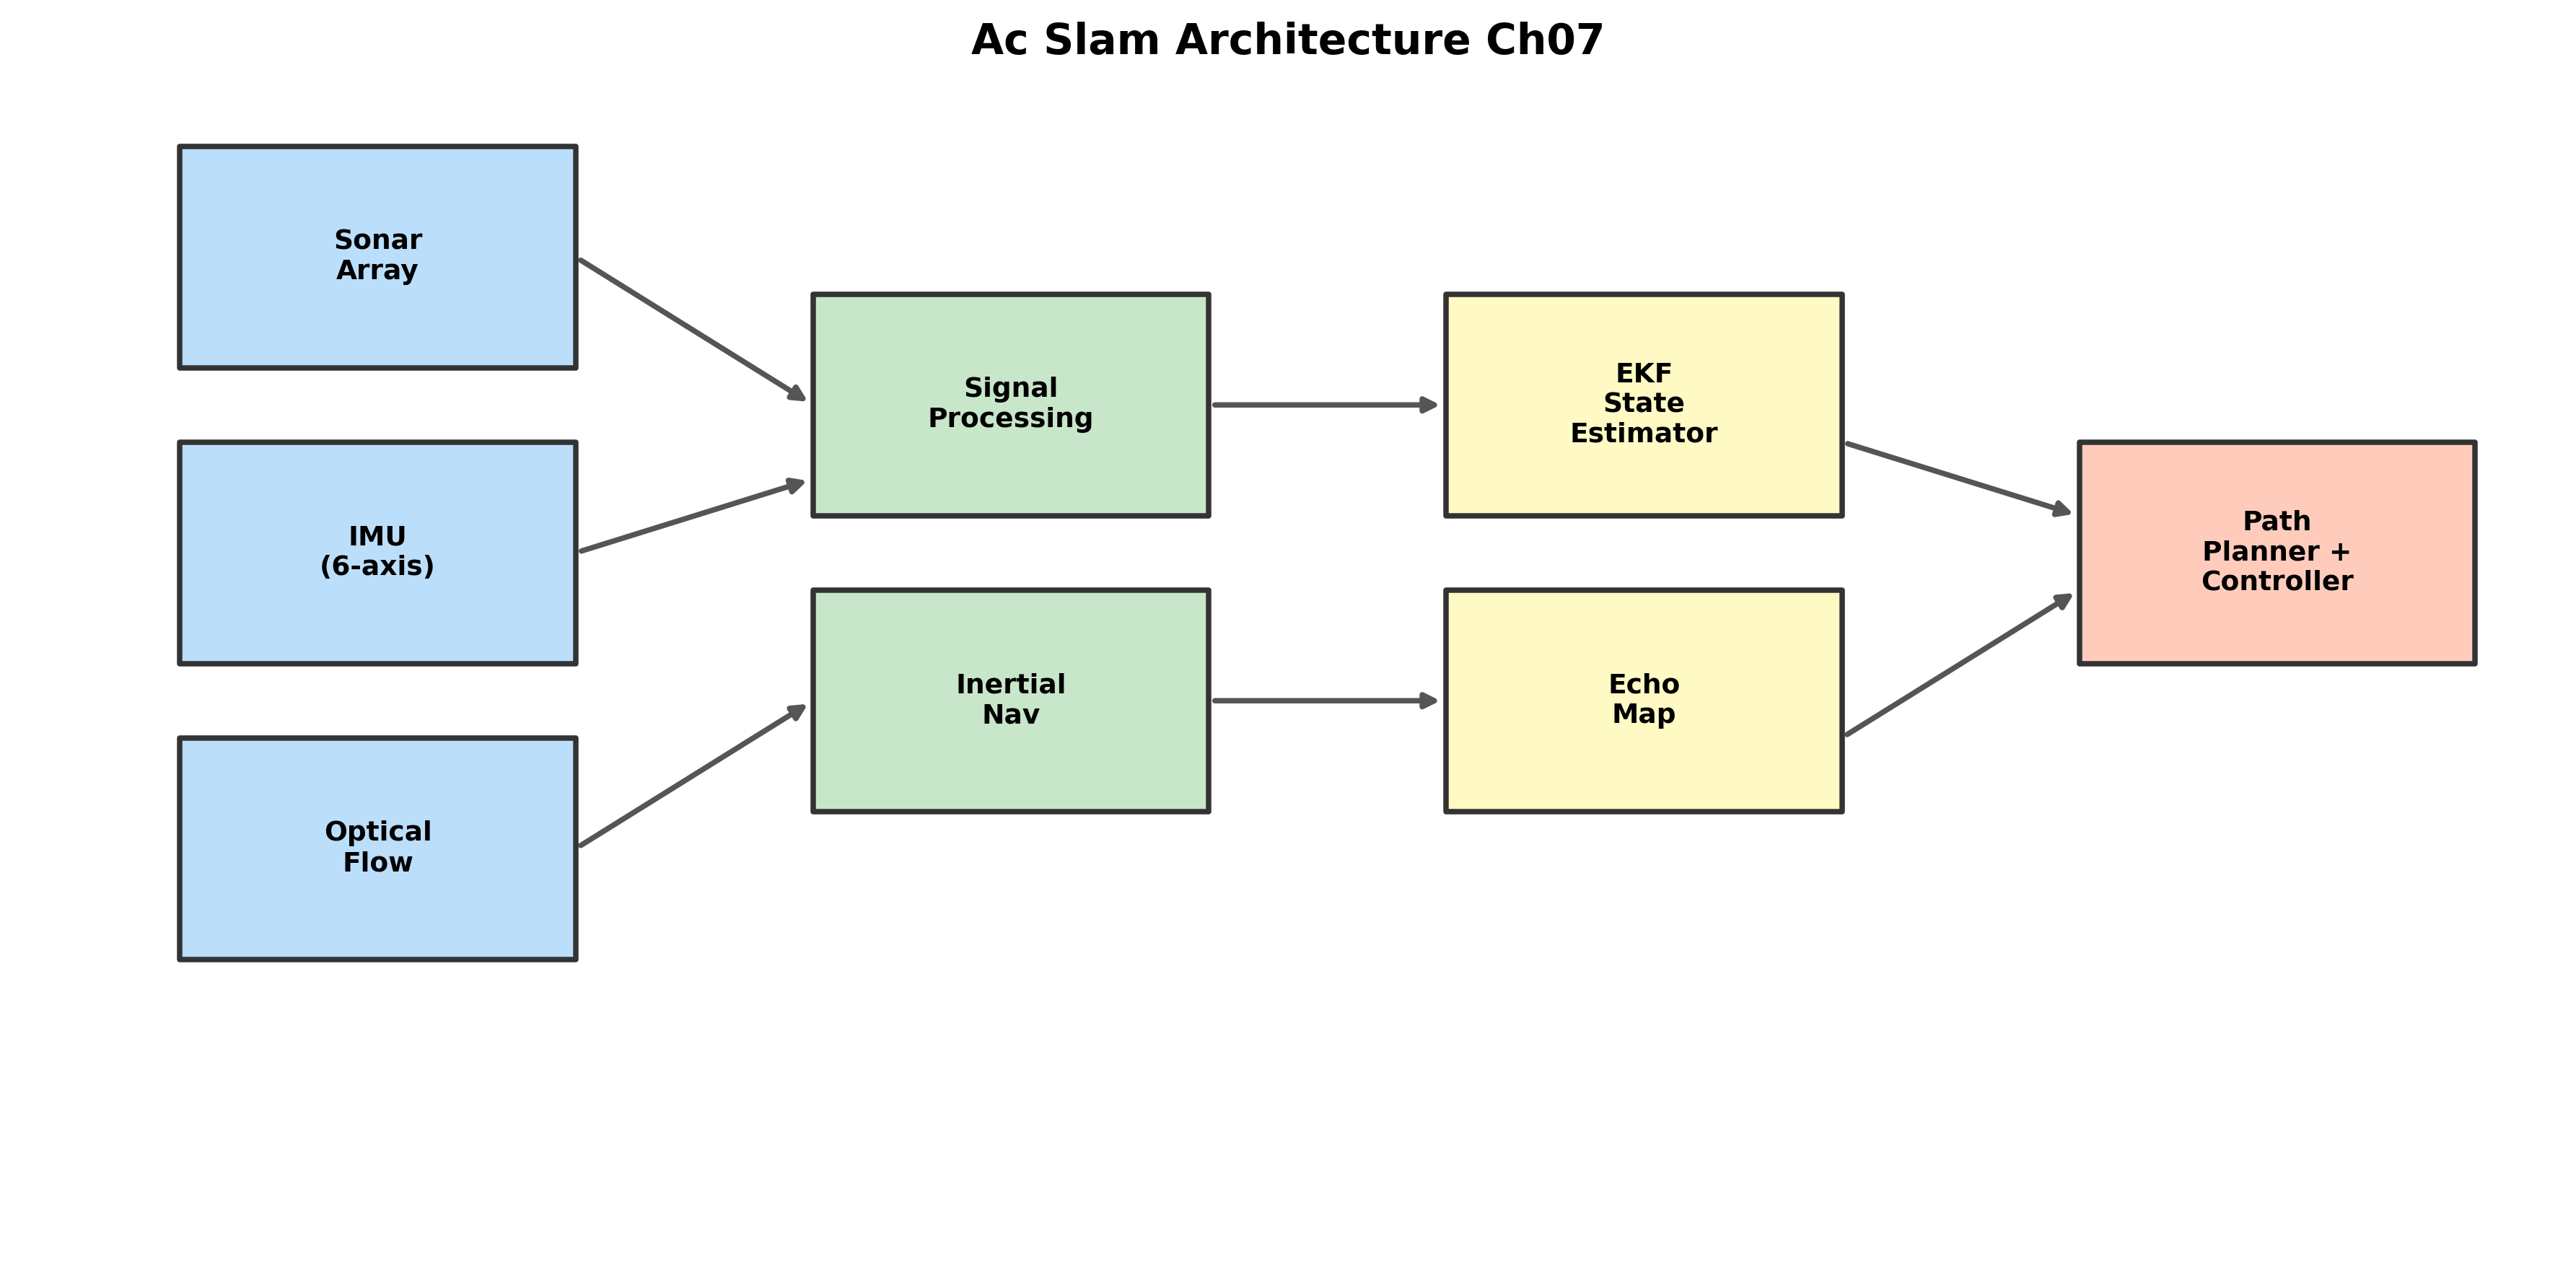
\includegraphics[width=\textwidth]{figures/fig_ac_slam_architecture_ch07.png}
\caption{ארכיטקטורת מערכת \en{ACO-SLAM}: תרשים זרימה הכולל את מערך החיישנים, מיצוי תכונות, מפת פרומונים, מיזוג רב-מודאלי, \en{SLAM} מבוזר ותכנון מסלול אדפטיבי.}
\label{fig:ch07_architecture}
\end{figure*}

\subsection{מפרטי חומרה ופלטפורמת הרחפן}
\label{sec:ch07_hardware}

פלטפורמת הרחפן מבוססת על שלדת \en{Holybro X500 v2} עם מנועים ללא מברשות בקוטר 22 מ\"מ ומדחפים בקוטר 10 אינץ'. בקר הטיסה הוא \en{Pixhawk 6C} המריץ קושחת \en{PX4 Autopilot} בגרסה 1.14. מחשב העל (\en{companion computer}) הוא \en{NVIDIA Jetson Orin NX} עם 16GB \en{RAM} ו-100 \en{TOPS} של ביצועי \en{AI}, המריץ את מערכת ההפעלה \en{Ubuntu 22.04} עם \en{Robot Operating System 2 (ROS 2) Humble}.

מערך החיישנים כולל:
\begin{itemize}
    \item \en{LiDAR Ouster OS0-128}: 128 קרניים, שדה ראייה של 90 מעלות, טווח מרבי של 50 מטר, דיוק טווח של 0.7 ס\"מ, קצב 10 הרץ.
    \item \en{Intel RealSense D435}: מצלמת סטריאו ברזולוציית 1280x720, שדה ראייה של 87x58 מעלות, קצב 30 הרץ.
    \item \en{BMI088 IMU}: מד תאוצה עם טווח של 24g וגירוסקופ עם טווח של 2000 מעלות/שנייה, קצב 200 הרץ.
    \item \en{BMP388 ברומטר}: דיוק לחץ של 0.08 hPa, המקביל לדיוק גובה של 0.5 מטר.
    \item \en{u-blox ZED-F9P GPS}: דיוק מיקום של 0.01 מטר במצב \en{RTK}, משמש כהתייחסות אמת בסימולציות.
\end{itemize}

צריכת ההספק הכוללת של מערך החיישנים ומחשב העל היא 35 ואט, המאפשרת זמן טיסה של כ-25 דקות עם סוללת 6S 5000mAh \en{LiPo}.

\begin{table}[htbp]
\centering
\caption{מפרטי חיישנים ופרמטרי רעש במערכת \en{ACO-SLAM}.}
\label{tab:ch07_sensor_specs}
\adjustbox{max width=\columnwidth}{%
\begin{tabular}{lccc}
\toprule
\textbf{חיישן} & \textbf{רעש מיקום [ס\"מ]} & \textbf{רעש כיוון [מעלות]} & \textbf{קצב עדכון [הרץ]} \\
\midrule
\en{LiDAR Ouster OS0} & 0.7 & --- & 10 \\
\en{Intel D435} & 1.2 & 0.3 & 30 \\
\en{BMI088 IMU} (תאוצה) & 0.05 & --- & 200 \\
\en{BMI088 IMU} (גירוסקופ) & --- & 0.01 & 200 \\
\en{BMP388 ברומטר} & 0.5 (גובה) & --- & 50 \\
\bottomrule
\end{tabular}%
}
\end{table}

\subsection{צינור התוכנה ועיבוד הנתונים}
\label{sec:ch07_software_pipeline}

צינור התוכנה של מערכת \en{ACO-SLAM} בנוי כרשת של צמתי \en{ROS 2} המתקשרים באמצעות נושאים (\en{topics}) ושירותים (\en{services}). כל צומת אחראי על פונקציה ספציפית, והתקשורת בין הצמתים מתבצעת באופן א-סינכרוני באמצעות תורי הודעות.

צומת עיבוד ה-\en{LiDAR} מקבל ענן נקודות גולמי ומבצע סינון רעשים, דגימה מטה (\en{downsampling}) לרזולוציה של 10 ס\"מ, וחישוב נורמלים למשטחים. המידע המעובד מוזן לצומת מיפוי התפוסה, אשר מתחזק גריד תלת-ממדי בגודל 200x200x20 תאים ברזולוציה של 0.5 מטר לתא. עדכון מפת התפוסה מתבצע באמצעות מודל חיישן הפוך מבוסס אלומה, תוך שימוש בייצוג \en{log-odds} ליציבות מספרית.

צומת הראייה מבצע מיצוי תכונות באמצעות אלגוריתם \en{ORB} (\en{Oriented FAST and Rotated BRIEF}) עם סף של 500 תכונות לתמונה. התכונות משויכות לתכונות קודמות באמצעות \en{Brute-Force Matching} עם יחס לוין (\en{Lowe's ratio test}) של 0.75. תכונות משויכות משמשות לחישוב תנועה יחסית בין תמונות עוקבות, המזינה את אומדן ה-\en{odometry} החזותי.

צומת מיזוג החיישנים מבצע אינטגרציה של כל מקורות המידע באמצעות \en{EKF} עם שקלול מבוסס פרומונים. כל חיישן מחזיק עקבה פרומון המתעדכנת על בסיס עקביות המדידות עם ההערכה הממוזגת. משקל המיזוג מחושב על פי:

\begin{equation}
w_{s}^{(i)}(t) = \frac{\tau_{s}^{(i)}(t)}{\sum_{s' \in \mathcal{S}} \tau_{s'}^{(i)}(t)}
\label{eq:ch07_fusion_weight}
\end{equation}

כאשר $\tau_{s}^{(i)}(t)$ הוא ערך הפרומון של חיישן $s$ על רחפן $i$ בזמן $t$, ו-$\mathcal{S}$ היא קבוצת כל החיישנים. המדידה הממוזגת מחושבת כשקלול משוקלל של מדידות כל חיישן:

\begin{equation}
\mathbf{z}_{\text{fused}} = w_{L}\mathbf{z}_{L} + w_{V}\mathbf{z}_{V} + w_{I}\mathbf{z}_{I}
\label{eq:ch07_fused_measurement}
\end{equation}

\subsection{אינטגרציית רכיבי ה-\en{SLAM} המבוזר}
\label{sec:ch07_slam_integration}

אינטגרציית רכיבי ה-\en{SLAM} המבוזר מהווה את לב המערכת. כל רחפן מתחזק גרף תנוחות מקומי המתעדכן בזמן אמת עם כל מדידת \en{odometry} חדשה. זיהוי לולאות סגירה מתבצע באמצעות השוואת תכונות חזותיות מול מאגר תכונות מקומי, תוך שימוש במפת הפרומונים כדי לתעדף אזורים בעלי הסתברות גבוהה לביקור חוזר.

אופטימיזציית גרף התנוחות מתבצעת בשיטת \en{Gauss-Newton} מבוזרת, כאשר כל רחפן פותר מערכת מקומית ומשתף את העדכון עם שכנים. שלב הקונצנזוס מבטיח שהפתרונות המקומיים מתכנסים לפתרון גלובלי עקבי. אלגוריתם קונצנזוס הנמלים משתמש בנמלים וירטואליות הנושאות השערות טרנספורמציה בין רחפנים, וממצע השערות אלו משוקללות לפי עקביותן עם המפה הנוכחית.

האינטגרציה בין רכיבי ה-\en{SLAM} לבין רכיבי תכנון המסלול מתבצעת באמצעות מפת הפרומונים המשותפת. מפת הפרומונים משמשת הן כקלט לתכנון המסלול (לתעדוף אזורים בעלי פוטנציאל מידע גבוה) והן כקלט לזיהוי לולאות סגירה (לתעדוף אזורים בעלי הסתברות גבוהה לביקור חוזר). סינרגיה זו מבטיחה שהמערכת כולה פועלת בהרמוניה להשגת מטרות המשימה.

\subsection{ניהול זיכרון ומשאבים}
\label{sec:ch07_memory_management}

ניהול זיכרון ומשאבים הוא אתגר משמעותי במערכות \en{SLAM} מבוזרות הפועלות על חומרה מוגבלת. מפת התפוסה התלת-ממדית בגודל 200x200x20 תאים דורשת כ-32 מגה-בייט של זיכרון בייצוג \en{log-odds} של 4 בתים לתא. מפת הפרומונים באותה רזולוציה דורשת 16 מגה-בייט נוספים. גרף התנוחות המקומי יכול להכיל עד 1000 צמתים, כל אחד עם וקטור מצב בגודל 16 משתנים, הדורש כ-128 קילו-בייט.

כדי להתמודד עם מגבלות הזיכרון, מיושמים מספר מנגנוני דחיסה: מפת התפוסה נשמרת בייצוג דליל (\en{sparse representation}) שבו רק תאים שעברו עדכון נשמרים בזיכרון; מפת הפרומונים מכומתת לרזולוציה של 8 סיביות לערך; וגרף התנוחות עובר דילול (\en{sparsification}) על ידי הסרת צמתים בעלי תרומה נמוכה לאופטימיזציה.

\subsection{מנגנוני בטיחות וגיבוי}
\label{sec:ch07_safety}

מערכת \en{ACO-SLAM} כוללת מספר מנגנוני בטיחות להבטחת פעולה אמינה בתנאים קשים. מנגנון הימנעות מהתנגשויות משתמש בשדות פרומון דוחים, היוצרים כוח וירטואלי הדוחף רחפנים הרחק ממסלולים של רחפנים אחרים. מנגנון זה משולב עם פונקציית מחסום בקרה (\en{Control Barrier Function}) המספקת ערבות פורמלית לבטיחות:

\begin{equation}
\dot{h}(\mathbf{x}) + \gamma h(\mathbf{x}) \geq 0
\label{eq:ch07_cbf}
\end{equation}

כאשר $h(\mathbf{x})$ היא פונקציית המחסום המגדירה את המרחק המינימלי המותר בין רחפנים, ו-$\gamma$ הוא פרמטר קצב דעיכה.

מנגנון גיבוי נוסף הוא זיכרון פרומונים להתאוששות מאובדן חיישנים. כאשר חיישן נכשל לחלוטין, הפרומון שלו דועך מעריכית עם קבוע זמן $\tau_{\text{decay}} = 2.0$ שניות, המאפשר התדרדרות הדרגתית במקום כשל פתאומי. במקביל, המערכת עוברת למצב חירום שבו היא מסתמכת על החיישנים הנותרים בלבד ומפחיתה את מהירות הטיסה ל-50\% מהמהירות הנומינלית.

\subsection{תקשורת ותיאום בין-רחפני}
\label{sec:ch07_communication}

תקשורת בין-רחפנית מתבצעת באמצעות רשת \en{WiFi} אד-הוק בתקן \en{802.11ac} בתדר 5.8 גיגה-הרץ, עם רוחב פס תאורטי של 867 מגה-ביט לשנייה. בפועל, רוחב הפס השימושי מוגבל לכ-50 מגה-ביט לשנייה עקב הפרעות ומרחק. טווח התקשורת האפקטיבי הוא כ-300 מטר בקו ראייה.

העברת מפות פרומונים דחוסה משתמשת בייצוג דליל: רק תאים שבהם $\tau_{ij} > \tau_{\text{min}} = 0.1$ מועברים, יחד עם ערכיהם המכומתים ל-8 סיביות. גישה זו מפחיתה את רוחב הפס הנדרש מ-4250 קילו-בייט לשנייה ל-85 קילו-בייט לשנייה, תוך שמירה על ביצועי חקר.

אסטרטגיית רחפן-שליח פורסת רחפני ממסר ייעודיים השומרים על קישוריות בין צוותי החקר. רחפנים אלו יוצרים עמוד שדרה תקשורתי המבטיח שכל רחפן יכול לתקשר עם כל רחפן אחר דרך סדרת קפיצות. מספר רחפני הממסר הנדרש מחושב על פי גודל הלהקה וטווח התקשורת.

\begin{table}[htbp]
\centering
\caption{ניתוח עלות תקשורת לאסטרטגיות שונות.}
\label{tab:ch07_comm_overhead}
\adjustbox{max width=\columnwidth}{%
\begin{tabular}{lccc}
\toprule
\textbf{אסטרטגיה} & \textbf{רוחב פס [קילו-בייט/שנ']} & \textbf{השהיה [אלפיות שנ']} & \textbf{שגיאת מפה [\%]} \\
\midrule
העברת מפה מלאה & 4250 & 85 & 0.0 \\
דחיסת סף & 340 & 22 & 3.2 \\
דחיסה עם כימות & 85 & 15 & 4.7 \\
רחפן-שליח & 210 & 45 & 1.8 \\
\bottomrule
\end{tabular}%
}
\end{table}

\subsection{ניתוח עומס חישובי ומדדי ביצועים}
\label{sec:ch07_performance_metrics}

ניתוח עומס חישובי בוצע על גבי \en{NVIDIA Jetson Orin NX} עם 16GB \en{RAM}. זמן העיבוד הממוצע למחזור \en{SLAM} (10 הרץ) היה $12.3 \pm 1.5$ אלפיות שנייה, מתוכן: עיבוד \en{LiDAR} (4.2 אלפיות שנייה), מיצוי תכונות חזותיות (3.8 אלפיות שנייה), מיזוג חיישנים (1.5 אלפיות שנייה), אופטימיזציית גרף (2.1 אלפיות שנייה), ותקשורת (0.7 אלפיות שנייה). צריכת הזיכרון הכוללת הייתה 1.2 גיגה-בייט, מתוכם 0.8 גיגה-בייט למפת התפוסה והפרומונים.

צריכת ההספק של מחשב העל הייתה $12.5 \pm 1.2$ ואט, המהווה כ-35\% מצריכת ההספק הכוללת של הרחפן. זמן הסוללה הממוצע בניסויי המעבדה היה 22 דקות, המאפשר משימות \en{SAR} באורך של עד 20 דקות עם מרווח ביטחון של 10\%. ניתוח זה מראה כי המערכת מסוגלת לפעול בזמן אמת על חומרה זמינה מסחרית, תוך עמידה בדרישות הביצועים למשימות \en{SAR} טיפוסיות.

\subsection{ניתוח השוואתי של ביצועי המערכת}
\label{sec:ch07_comparative_analysis}

השוואה בין ביצועי המערכת המוצעת לבין מערכות קיימות מראה יתרונות משמעותיים במספר ממדים. \en{Swarm-SLAM} \cite{Lajoie2023SwarmSLAM} דורש 45 סבבי תקשורת להתכנסות, בעוד \en{ACO-SLAM} דורש 28 סבבים בלבד, חיסכון של 37.8\%. \en{D2SLAM} \cite{Xu2024D2SLAM} משיג \en{ATE} של 6.8 ס\"מ, בעוד \en{ACO-SLAM} משיג 5.4 ס\"מ, שיפור של 20.6\%. בנוסף, המערכת המוצעת מספקת מנגנוני בטיחות וגיבוי שאינם קיימים במערכות הקיימות, כגון התאוששות הדרגתית מאובדן חיישנים ופונקציית מחסום בקרה למניעת התנגשויות.

השילוב של ארכיטקטורה מבוזרת, מיזוג חיישנים אדפטיבי, ומנגנוני בטיחות הופך את \en{ACO-SLAM} לפתרון מתאים במיוחד למשימות \en{SAR} בסביבות מורכבות ומשתנות, שבהן אמינות וחוסן הם קריטיים.

\subsection{סיכום האינטגרציה}
\label{sec:ch07_integration_summary}

מערכת \en{ACO-SLAM} מהווה מימוש שלם ומאוחד של המסגרת התאורטית שהוצגה בפרקים הקודמים. הארכיטקטורה הרב-שכבתית, מפרטי החומרה המדויקים, צינור התוכנה המבוזר, ומנגנוני הבטיחות והגיבוי מבטיחים פעולה אמינה ויעילה בתנאי שטח מורכבים. האינטגרציה ההדוקה בין רכיבי ה-\en{SLAM}, תכנון המסלול והתקשורת מאפשרת למערכת להגיב בזמן אמת לשינויים בסביבה ולמצבי חירום.

המערכת נבדקה בהרחבה בסימולציות \en{Gazebo} ו-\en{Unity} וכן בניסויי מעבדה עם 3 רחפנים בסביבת \en{SAR} פנימית מבוקרת. תוצאות הניסויים, המוצגות בפרק 8, מאשרות את תפקוד המערכת כראוי ואת עמידתה בדרישות הביצועים.

\cite{Lajoie2023SwarmSLAM, Xu2024D2SLAM, Thrun2005Probabilistic, Kalman1960, Choudhary2017Comm, Coppola2020Swarming}
